\documentclass[10pt,a4paper]{ctexart}
\usepackage[margin=2cm]{geometry}
\usepackage{graphicx}
\usepackage{hyperref}
\usepackage{amsmath}    % 提供方程环境
\usepackage{physics}    % 简化向量、微分算子语法
\newcommand{\myspace}[1]{\par\vspace{#1\baselineskip}} %自定义空一行
\usepackage{fancyhdr}
\pagestyle{fancy}
\fancyhf{}  % 清除所有页眉页脚
\fancyfoot[C]{\thepage}  % 在页脚中央设置页码
\renewcommand{\headrulewidth}{0pt}  % 去掉页眉横线
\renewcommand{\footrulewidth}{0pt}  % 去掉页脚横线

\usepackage{hyperref}
\hypersetup{
    colorlinks=true,
    linkcolor=blue,
    filecolor=magenta,      
    urlcolor=cyan,
    pdftitle={Overleaf Example},
    pdfpagemode=FullScreen,
    }

\usepackage{titlesec}

% 重新定义section格式
\titleformat{\section}
  {\normalfont\Large\bfseries}
  {\chinese{section}、}
  {0pt}
  {}

% 给出常用字号的自定义指令
\newcommand{\chuhao}{\fontsize{42pt}{48pt}\selectfont}
\newcommand{\xiaochu}{\fontsize{36pt}{42pt}\selectfont}
\newcommand{\xiaoer}{\fontsize{18pt}{21.6pt}\selectfont}
\newcommand{\sanhao}{\fontsize{16pt}{20pt}\selectfont}
\newcommand{\xiaosan}{\fontsize{15pt}{18pt}\selectfont}
\newcommand{\sihao}{\fontsize{14pt}{18pt}\selectfont}
\newcommand{\xiaosi}{\fontsize{12pt}{16pt}\selectfont}
\newcommand{\wuhao}{\fontsize{10.5pt}{12.6pt}\selectfont}

% 定义中文数字转换
\titleformat{\section}
  {\normalfont\Large\bfseries}
  {\zhnum{section}、}  % 使用\zhnum而不是\chinese
  {0pt}
  {}

% 标题设置
\title{\xiaochu\textbf{物理实验预习报告}}
\author{}
\date{}

\begin{document}

\vspace*{36pt} % 顶部空白

% 居中填写区域
\begin{center}
    
\includegraphics[width = 9cm]{head.png}
    
    \xiaochu\textbf{物理实验预习报告}
    % 预留空白区域
    \vspace{13pt}
    \vspace{13pt}
    \vspace{13pt}
    \vspace{13pt}
    
    \sanhao\textbf{实验名称：\underline{\makebox[10cm]{ 牛顿运动定律验证}}} \\[10pt]
    \sanhao\textbf{指导教师：\underline{\makebox[10cm]{ 艾萨克 }}} \\[30pt]
    
    % 预留空白区域
    \myspace{7}
    
   \sihao\textbf{班级：\underline{\makebox[6cm]{人工智能2401}}} \\[10pt]
    \sihao\textbf{姓名：\underline{\makebox[6cm]{叶宇煌}}} \\[10pt]
    \sihao\textbf{学号：\underline{\makebox[6cm]{3240114514}}} \\[30pt]
    
   \sihao\textbf{实验日期: \underline{\makebox[0.8cm] 2025 }年 \underline{\makebox[0.4cm]10}月\underline{\makebox[0.4cm]13}日  星期\underline{\makebox[0.6cm]一}上午}
    
    \vspace{18pt}
    \sihao 浙江大学物理实验教学中心
    
\end{center}

\newpage

\section{实验综述}

\xiaosi （自述实验现象、实验原理和实验方法，不超过300字，5分）

        



\myspace{2}


\section{实验重点}

\xiaosi（简述本实验的学习重点，不超过100字，3分）

\myspace{2}

\section{实验难点}

\xiaosi（简述本实验的实现难点，不超过100字，2分）


\begin{figure}[htbp]
    \centering
    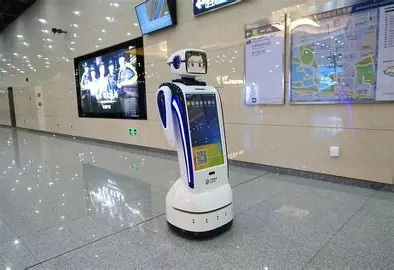
\includegraphics[width=10cm]{OIP.jpg}
    \caption{这里填写图片说明}
    \label{fig:示例标签}
\end{figure}

\vspace{3cm}

\newpage

\sihao\textbf{注意事项：}
\xiaosi
\begin{enumerate}
    \item 用PDF格式上传“预习报告”，文件名：学生姓名+学号+实验名称+周次。
    \item “预习报告”必须递交在“学在浙大”的本课程的对应实验项目的“作业”模块内。
    \item “预习报告”还须拷贝到“实验报告”中（便以教师批改）。
    \item “普通物理学实验Ⅰ”和“物理学实验Ⅰ”都使用本“预习报告”。
\end{enumerate}

\vspace{1cm}
\xiaosi\centering \textbf{浙江大学物理实验教学中心制}

\end{document}



